\documentclass[11pt,oneside]{article}

	% History ================================================================
	% 2023.06.03 - Modified from Chase Murray's version
	% ========================================================================

    % STANDARD PACKAGES ======================================================
    \usepackage{datetime}
    \usepackage{graphicx}
    % \usepackage{ctex} % Allow Chinese characters
    \usepackage[utf8]{inputenc}
    \usepackage[american]{babel}
    \usepackage{amssymb}
    \usepackage[intlimits]{amsmath}
    \usepackage{amsfonts}
    \usepackage{amsthm}
    \usepackage{array}
    \usepackage{mdwlist}        
    \usepackage[labelsep=quad,indention=10pt]{subfig}
    \usepackage{algorithm}
    \usepackage[noend]{algpseudocode}
    \usepackage{lscape}
    \usepackage{rotating} % Allows \begin{sideways} \end{sideways} for vertical table headers.    
    \usepackage{threeparttable} % Allow footnotes in tables.    
    \usepackage{tabularx}
    \usepackage{multirow} % Allow table cells to span multiple rows/cols.
    \usepackage{makecell}
    \usepackage{longtable}
    \usepackage{url} % Allow \url{} and \href{url}{name}
    \usepackage{verbatim}    
    \usepackage{enumerate} % http://www.tex.ac.uk/cgi-bin/texfaq2html?label=enumerate
    \usepackage{color} % Allow colored fonts
    \usepackage[toc,page]{appendix}

    \usepackage{bm}

    \usepackage{tikz}
    \usepackage{diagbox}
    \usepackage{lastpage} % \pageref{LastPage} = total number of pages.
    \usepackage{ifthen}        
    \usepackage{setspace} % Allows \singlespacing, \onehalfspacing, \doublespacing 
    \usepackage{listings} % Allows formatting of Python code (and other languages)
    \usepackage{wrapfig}
    \usepackage[normalem]{ulem} % Allows strikethrough (\sout{text to strike})
    % \usepackage{subfigure}        % Allows subfigs/subfloats


    \usepackage{xcolor,colortbl}    % http://ctan.org/pkg/xcolor
    % \usepackage[table]{xcolor}    % https://tex.stackexchange.com/questions/50349/color-only-a-cell-of-a-table
    
    % Make sure that {color} and {xcolor} are called before mdframed
    \usepackage[framemethod=TikZ]{mdframed}    % Allows colored textbox

    \usepackage{lipsum}                     % Dummy text
    % ========================================================================

    % DEFINE PROGRAMMING FORMAT ++++++++++++++++++++++++++++++++++++++++++++++
        \lstset{language=Python}          % Set your language (you can change the language for each code-block optionally)

        \definecolor{mygreen}{rgb}{0,0.6,0}
        \definecolor{mygray}{rgb}{0.5,0.5,0.5}
        \definecolor{mymauve}{rgb}{0.58,0,0.82}

        \lstset{
          backgroundcolor=\color{gray!05!white},   % choose the background color; you must add \usepackage{color} or \usepackage{xcolor}; should come as last argument
          basicstyle=\ttfamily,                    % the size of the fonts that are used for the code
          breakatwhitespace=false,                 % sets if automatic breaks should only happen at whitespace
          breaklines=true,                         % sets automatic line breaking
          captionpos=t,                            % sets the caption-position to bottom
          commentstyle=\color{black},              % comment style
          deletekeywords={...},                    % if you want to delete keywords from the given language
          escapeinside={\%*}{*)},                  % if you want to add LaTeX within your code
          extendedchars=true,                      % lets you use non-ASCII characters; for 8-bits encodings only, does not work with UTF-8
          frame=single,                               % adds a frame around the code
          keepspaces=true,                         % keeps spaces in text, useful for keeping indentation of code (possibly needs columns=flexible)
          % keywordstyle=\color{blue},             % keyword style
          language=Python,                         % the language of the code
          morekeywords={*,...},                    % if you want to add more keywords to the set
          numbers=left,                            % where to put the line-numbers; possible values are (none, left, right)
          numbersep=5pt,                           % how far the line-numbers are from the code
          % numberstyle=\tiny\color{mygray},       % the style that is used for the line-numbers
          rulecolor=\color{black},                 % if not set, the frame-color may be changed on line-breaks within not-black text (e.g. comments (green here))
          showspaces=false,                        % show spaces everywhere adding particular underscores; it overrides 'showstringspaces'
          showstringspaces=false,                  % underline spaces within strings only
          showtabs=false,                          % show tabs within strings adding particular underscores
          stepnumber=1,                            % the step between two line-numbers. If it's 1, each line will be numbered
          % stringstyle=\color{mymauve},           % string literal style
          tabsize=4,                               % sets default tabsize to 2 spaces
          % title=\lstname,                        % show the filename of files included with \lstinputlisting; also try caption instead of title
          xleftmargin=35pt,
          xrightmargin=15pt, 
          aboveskip=0pt,
          belowskip=5pt
        }
    % ++++++++++++++++++++++++++++++++++++++++++++++++++++++++++++++++++++++++

    % DEFINE/RENEW SOME ENVIRONMENTS =========================================    
        \renewenvironment{abstract}
          {\normalfont\footnotesize
            \list{}{\labelwidth0pt
              \leftmargin20pt \rightmargin\leftmargin
              \listparindent\parindent \itemindent0pt
              \parsep0pt
              \let\fullwidthdisplay\relax
            }
            \item[\hskip\labelsep\bfseries\abstractname:] %
        }{
          \endlist}

        \newcommand{\keywordsname}{Keywords}
        \newenvironment{keywords}
          {\normalfont\footnotesize
            \list{}{\labelwidth0pt
              \leftmargin20pt \rightmargin\leftmargin
              \listparindent\parindent \itemindent0pt
              \parsep0pt
              \let\fullwidthdisplay\relax}
            \item[\hskip\labelsep\bfseries\keywordsname:]}{\endlist}

        \newcommand{\dochistname}{History}
        \newenvironment{DocHistory}
          {\normalfont\footnotesize
            \list{}{\labelwidth0pt
              \leftmargin20pt \rightmargin\leftmargin
              \listparindent\parindent \itemindent0pt
              \parsep0pt
              \let\fullwidthdisplay\relax}
            \item[\hskip\labelsep\bfseries\dochistname:]}{\endlist}
    % ========================================================================    

    % DEFINE PAGE FORMATTING +++++++++++++++++++++++++++++++++++++++++++++++++
        % Select Line Spacing:
        \singlespacing
        % \onehalfspacing        
        % \doublespacing    

        % Margins:
        \usepackage[letterpaper,left=1.0in,top=1.0in,right=1.0in,bottom=1.0in]{geometry}
    
        % Page Style
        \pagestyle{plain}    % Includes page number
        %\pagestyle{empty}    % Completely blank                

        % By default all math is set to inline mode. The \displaystyle command
        % ensures that we don't get small fractions or summations with limits
        % on the sides.
        \everymath{\displaystyle}    
        
        % http://tex.stackexchange.com/questions/5223/command-for-argmin-or-argmax
        \DeclareMathOperator*{\argmin}{arg\,min}

        % Allow flalign items to be split over multiple pages:
        \allowdisplaybreaks[1]   % See ftp://ftp.ams.org/pub/tex/doc/amsmath/amsldoc.pdf    
    % ++++++++++++++++++++++++++++++++++++++++++++++++++++++++++++++++++++++++

    % DEFINITION, THEOREM, AND LEMMA +++++++++++++++++++++++++++++++++++++++++

        \theoremstyle{definition}
            \newtheorem{definition}{Definition}[section]
            \newtheorem*{example}{Example}
            \newtheorem{problem}{Problem}[section]
            \newtheorem*{solution}{Solution}
            \newtheorem{hypothesis}{Hypothesis}[section]
        \theoremstyle{plain}
            \newtheorem{theorem}{Theorem}[section]
            \newtheorem{corollary}{Corollary}[theorem]
            \newtheorem{lemma}[theorem]{Lemma}
            \newtheorem{conjecture}{Conjecture}
            \newtheorem{proposition}{Proposition}
        \theoremstyle{remark}
            \newtheorem*{remark}{Remark}

    % ++++++++++++++++++++++++++++++++++++++++++++++++++++++++++++++++++++++++

    % CUSTOM MACROS ++++++++++++++++++++++++++++++++++++++++++++++++++++++++++

        % This is how you may create a new variable:
        % \newcommand{\docjunk}{ text to display }
        
        % See https://gist.github.com/benkehoe/c46647134d4bbd514869
        % for more examples.

        % Create a box marked ``To Do'' around text.
        % \todo{  insert text here  }.
        \newcommand{\todo}[1]{\vspace{5 mm}\par \noindent
        \marginpar{\textsc{to do}}
        \framebox{\begin{minipage}[c]{0.95 \textwidth}
        \tt\begin{center} #1 \end{center}\end{minipage}}\vspace{5 mm}\par}

        % Create an empty box marked ``Result'' in the margin.
        % Specify the number of empty rows.
        % \result{8 em}.
        \newcommand{\result}[1]{\vspace{5 mm}\par \noindent
        \marginpar{\textsc{Result}} $\qquad\qquad$
        \framebox{\begin{minipage}[c]{0.75 \textwidth}
        \tt\begin{center} \vspace{#1} \end{center}\end{minipage}}\vspace{5 mm}\par}

        % Color selected text in red font.
        % \alert{text to color}
        \newcommand{\alert}[1]{{\color{red}#1}}

        % Color selected text in blue font.
        % \edited{text to color}
        \newcommand{\edited}[1]{{\color{blue}#1}}

        % Color selected text and add a "FIXME" note in the margin.
        % \fixme{text to color}
        \newcommand{\fixme}[1]{{\color{red}#1}
            \marginpar{\textsc{\color{red}fixme}}}

        % Color selected text (optional) and add a note in brackets.
        % \note[selected text]{comments}
        % \note{comments}
        \renewcommand{\note}[2][]{
            {\color{blue}#1 %
            [\textsc{note}:~#2]}
        }
        
        % Color selected text (optional) and add a note from someone.
        % \notefrom[selected text]{from}{comments}
        % \notefrom{from}{comments}
        \newcommand{\notefrom}[3][]{
            {\color{green!50!black}#1 %
            [\textsc{from #2}:~#3]}
        }
        
        % Color selected text (optional) and add a note to someone.
        % \noteto[selected text]{to}{comments}
        % \noteto{to}{comments}
        \newcommand{\noteto}[3][]{
            {\color{red}#1 %
            [\textsc{to #2}:~#3]}
        }

        % Color and Line Settings for Boxed Text
        \mdfsetup{
        % middlelinecolor=red,
        middlelinewidth=1pt,
        % linecolor=blue,
        % linewidth=1pt,
        backgroundcolor=orange!10!white,
        linecolor=orange!50!black,
        roundcorner=5pt}
        
        % Shortcut for referencing figures/tables:
        % Usage:  \figref{fig:name} --> Figure 1.
        \newcommand{\figref}[1]{\figurename~\ref{#1}}
        \newcommand{\tabref}[1]{\tablename~\ref{#1}}
    % ++++++++++++++++++++++++++++++++++++++++++++++++++++++++++++++++++++++++

    % SETUP TikZ +++++++++++++++++++++++++++++++++++++++++++++++++++++++++++++
        \usetikzlibrary{arrows,shapes,matrix}
        \usetikzlibrary{decorations.pathmorphing} 
        \usepgflibrary{plotmarks}
        \usetikzlibrary{patterns}  
        \usetikzlibrary{positioning} 
        \usetikzlibrary{snakes}  
        \tikzstyle{block}=[draw opacity=0.7,line width=1.4cm]
        
        % MORE STUFF TO ADD HERE?
    % ++++++++++++++++++++++++++++++++++++++++++++++++++++++++++++++++++++++++

    % SETUP BIBLIOGRAPHY +++++++++++++++++++++++++++++++++++++++++++++++++++++
    % [This section MUST be used if you have a bibliography.    ]
    % [Otherwise, leave this section commented out.        ]
    % \begin{comment}

        % FIXME -- EXPLAIN
        
        % Setup the Bibliography Style -- Select ONE of the following:
        % \usepackage{natbib}
        % \usepackage[sectionbib,square]{natbib}     %%% See natbib.pdf for explanation.
        % \usepackage[sectionbib,round]{natbib}
        \usepackage[square,numbers]{natbib}

        \bibliographystyle{plainnat}

        % Natbib setup for author-year style
        % \bibpunct has 1 optional and 6 mandatory arguments:
        %  [0.] The character preceding a post-note, default is a comma plus space. In redefining this character, 
        %     one must include a space if one is wanted. 
        %  1. the opening bracket symbol, default = (
        %  2. the closing bracket symbol, default = )
        %  3. the punctuation between multiple citations, default = ;
        %  4. the letter `n' for numerical style, or `s' for numerical superscript style, 
        %    any other letter for author-year, default = author-year;
        %  5. the punctuation that comes between the author names and the year
        %  6. the punctuation that comes between years or numbers when common author lists are suppressed (default = ,);

        % Natbib setup for author-year style
        \bibpunct[, ]{(}{)}{,}{a}{}{,}                % Use author names
        % \bibpunct[, ]{[}{]}{,}{n}{}{,}            % Use numbers
        
        \def\bibfont{\small}
        \def\bibsep{\smallskipamount}
        \def\bibhang{24pt}
        \def\newblock{\ }
        \def\BIBand{and}
    % \end{comment}
    % ++++++++++++++++++++++++++++++++++++++++++++++++++++++++++++++++++++++++

    % DOCUMENT INFO ++++++++++++++++++++++++++++++++++++++++++++++++++++++++++
        \newcommand{\docTitle}{}

        % List authors here, separated by \and 
        \newcommand{\docAuthor}{}
        % \newcommand{\docAuthor}{}

        \newcommand{\docAffil}{
            School of Management, Shanghai University, Shanghai, China
        }

        \newcommand{\docAbstract}{}

        \newcommand{\docKeyword}{}

        % This date will appear under the title.
        \newcommand{\docDate}{\today}       % {} --> don't show a date.
            
        % This date will appear in the page header:
        \newcommand{\draftDate}{\today}    % {\today} --> draft, {} --> finalized (hidden)
    
        % The image files should be saved here:
        \graphicspath{ {../../image/} }
    % ++++++++++++++++++++++++++++++++++++++++++++++++++++++++++++++++++++++++

    % DEFINE HEADER ++++++++++++++++++++++++++++++++++++++++++++++++++++++++++
        \usepackage{fancyhdr}
        \pagestyle{fancy}
        \ifthenelse{\equal{\draftDate}{}}
            {
                % This is the final version...remove the date from the header
                \chead{}
            }
            {
                % This is a working draft...include the date in the header
                % \chead{\color{red}DRAFT -- Updated \draftDate~at~\currenttime}
            }
        \lhead{}    % no left/right header content
        \rhead{}
        %\cfoot{}
        %\lfoot{}
        %\rfoot{}
        \renewcommand{\headrulewidth}{0pt}
        \renewcommand{\footrulewidth}{0pt}
        %\fancyfoot{}
    % ++++++++++++++++++++++++++++++++++++++++++++++++++++++++++++++++++++++++
    
    % DEFINE PROGRAMMING FORMAT ++++++++++++++++++++++++++++++++++++++++++++++
    \lstset{language=Python}          % Set your language (you can change the language for each code-block optionally)

    \definecolor{mygreen}{rgb}{0,0.6,0}
    \definecolor{mygray}{rgb}{0.5,0.5,0.5}
    \definecolor{mymauve}{rgb}{0.58,0,0.82}

    \lstset{ %
      backgroundcolor=\color{gray!05!white},   % choose the background color; you must add \usepackage{color} or \usepackage{xcolor}; should come as last argument
      basicstyle=\ttfamily,        % the size of the fonts that are used for the code
      breakatwhitespace=false,         % sets if automatic breaks should only happen at whitespace
      breaklines=true,                 % sets automatic line breaking
      captionpos=t,                    % sets the caption-position to bottom
      commentstyle=\color{black},    % comment style
      deletekeywords={...},            % if you want to delete keywords from the given language
      escapeinside={\%*}{*)},          % if you want to add LaTeX within your code
      extendedchars=true,              % lets you use non-ASCII characters; for 8-bits encodings only, does not work with UTF-8
      frame=single,                       % adds a frame around the code
      keepspaces=true,                 % keeps spaces in text, useful for keeping indentation of code (possibly needs columns=flexible)
      % keywordstyle=\color{blue},       % keyword style
      language=Python,                 % the language of the code
      morekeywords={*,...},           % if you want to add more keywords to the set
      numbers=none,                    % where to put the line-numbers; possible values are (none, left, right)
      numbersep=5pt,                   % how far the line-numbers are from the code
      % numberstyle=\tiny\color{mygray}, % the style that is used for the line-numbers
      rulecolor=\color{black},         % if not set, the frame-color may be changed on line-breaks within not-black text (e.g. comments (green here))
      showspaces=false,                % show spaces everywhere adding particular underscores; it overrides 'showstringspaces'
      showstringspaces=false,          % underline spaces within strings only
      showtabs=false,                  % show tabs within strings adding particular underscores
      stepnumber=1,                    % the step between two line-numbers. If it's 1, each line will be numbered
      % stringstyle=\color{mymauve},     % string literal style
      tabsize=4,                       % sets default tabsize to 2 spaces
      % title=\lstname,                   % show the filename of files included with \lstinputlisting; also try caption instead of title
      xleftmargin=35pt,
      xrightmargin=15pt, 
      aboveskip=0pt,
      belowskip=5pt
    }
    % ++++++++++++++++++++++++++++++++++++++++++++++++++++++++++++++++++++++++

    \newcommand{\titleSec}{
        % See https://tex.stackexchange.com/questions/216098/redefine-maketitle
        \begin{center}
        % \let \footnote \thanks
        {\Large \textbf{\docTitle} \par}

        % Authors?
        % Comment these lines out if you want to hide authors
        \vskip 1.0em%
        \lineskip .5em%
        \begin{tabular}[t]{c}
            \docAuthor
        \end{tabular}\par%

        % Affiliation?
        % Comment these lines out if you want to hide affiliation info
        \vskip 1.0em%
        {\small \docAffil \par}

        % Displayed date?
        % Comment these lines out if you want to hide the date
        %\vskip 1.0em%
        %{\small \docDate \par}  

        \end{center}
        \par
        \vskip 1.5em

        % \begin{abstract}
        %     \docAbstract
        % \end{abstract}

        % \begin{keywords}
        %     \docKeyword
        % \end{keywords}

        % This is version \texttt{\templateVersion} of this template.
        % Visit \templatesURL for the latest versions.
    }
\usepackage{makecell}
% \setlength{\parindent}{0pt}
\usepackage{float}
\newcommand{\floor}[1]{\left\lfloor #1 \right\rfloor}
\newcommand{\ceil}[1]{\left\lceil #1 \right\rceil}

\usetikzlibrary{shapes.geometric, arrows}
    \tikzstyle{startstop} = [rectangle, rounded corners, minimum width=3cm, minimum height=1cm,text centered, draw=black]
    \tikzstyle{io} = [trapezium, trapezium left angle=70, trapezium right angle=110, minimum width=3cm, minimum height=1cm, text centered, draw=black]
    \tikzstyle{process} = [rectangle, minimum width=2cm, minimum height=1cm, text centered, draw=black, inner sep=0.1cm]
    \tikzstyle{decision} = [diamond, minimum width=2cm, minimum height=0cm, text centered, draw=black, inner sep=0cm]
    \tikzstyle{arrow} = [thick,->,>=stealth]
    \tikzstyle{branchnode} = [circle, minimum size = 1cm, text centered, draw=black, inner sep=0.1cm]

\renewcommand{\docTitle}{Lecture 4 - Polyhedral Analysis and Cutting Plane Method}
\renewcommand{\docAuthor}{Lan Peng, Ph.D.}
\renewcommand{\docAffil}{School of Management, Shanghai University, Shanghai, China}
\begin{document}
    \titleSec

    \begin{center}
        \textit{``Life is a Crystal.''}
    \end{center}
    \section{Preliminaries}
        \subsection{Valid Inequalities and Faces}
            The inequality denoted by $(\pi, \pi_o)$ is called a valid inequality for $P$ if $\pi x \le \pi_0, \forall x \in P$. Note that $(\pi, \pi_0)$ is a valid inequality iff $P$ lies in the half-space $\{x\in \mathbb{R}^n|Ax\le b\}$

            \begin{figure}[H]
            \centering
            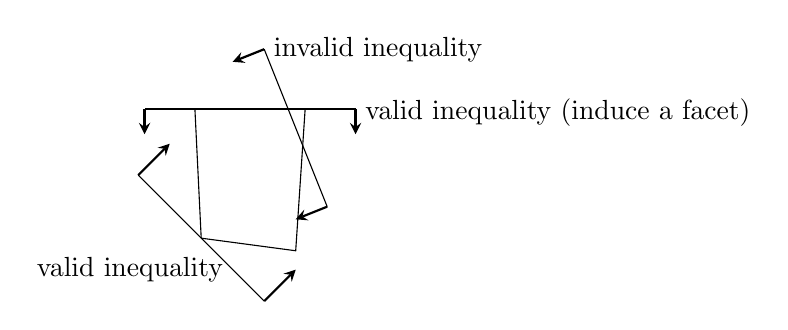
\begin{tikzpicture}[scale=0.4]
                \draw (0,0) -- (3, -0.4) -- (3.3, 4.1) -- (-0.2, 4.1) -- (0, 0);
                \draw (-2, 2) -- (2, -2);
                \draw (4.9, 4.1) -- (-1.8, 4.1);
                \draw (4, 1) -- (2, 6);
                \draw [arrow] (-1.8, 4.1) -> (-1.8, 3.3);
                \draw [arrow] (4.9, 4.1) -> (4.9, 3.3);
                \draw [arrow] (-2, 2) -> (-1, 3);
                \draw [arrow] (2, -2) -> (3, -1);
                \draw [arrow] (4, 1) -> (3, 0.6);
                \draw [arrow] (2, 6) -> (1, 5.6);
                \node at (1, -1) [left] {valid inequality};
                \node at (4.9, 4) [right] {valid inequality (induce a facet)};
                \node at (2, 6) [right] {invalid inequality};
            \end{tikzpicture}
            \caption{Example of valid/invalid inequality}
            \end{figure}

            \begin{itemize}
                \item If $(\pi, \pi_0)$ is a valid inequality for $P$ and $F=\{x\in P|\pi x=x_0\}$, $F$ is called a facet of $P$ and we say that $(\pi, \pi_0)$ represents or defines $F$
                \item A face is said to be proper if $F\ne \emptyset$ and $F\ne P$
                \item The face represented by $(\pi, \pi_0)$ is nonempty iff $\max \{\pi x |x\in P\}=\pi_0$
                \item If the face $F$ is nonempty, we say it supports $P$
                \item Let $P$ be a polyhedron with equality set $M^=$. If
                    \begin{equation*}
                        F=\{x\in P | \pi^T x = \pi_0\}
                    \end{equation*}
                    is not empty, then $F$ is a polyhedron. Let 
                    \begin{equation*}
                        M^= \subseteq M_F^=, M_F^{\le}=M \setminus M_F^= 
                    \end{equation*}
                    then 
                    \begin{equation*}
                        F=\{x | a_i^T x=b_i, \forall i \in M_F^=, a_i^T x \le b_i, \forall i \in M_f^{\le}\}
                    \end{equation*}
            \end{itemize}

        \subsection{Facet}
            \begin{itemize}
                \item A face $F$ is said to be a facet of $P$ if $dim(F) = dim(P)-1$
                \item Facets are all we need to describe polyhedral
                \item If $F$ is a facet of $P$, then in any description of $P$, there exists some inequality representing $F$
                \item Every inequality that represents a face that is not a facet is unnecessary in the description of $P$
                \item Every full-dimensional polyhedron $P$ has a unique (up to scalar multiplication) representation that consists of one inequality representing each facet of $P$
                \item If $dim(P) = n-k$ with $k>0$, then $P$ is described by a maximal set of linearly independent rows of $(A^=, b^=)$, as well as one inequality representing each facet of $P$
            \end{itemize}
            
        \subsection{Proving Facet}
            To prove an inequality $\sum_i a_i x_i \le b_i$ is facet inducing for a $D$ dimensional polyhedral, we need to prove there are $D$ affinely independent vectors in $\sum_i a_i x_i = b_i$

    \section{Some Examples}
        \subsection{Vertices Packing}
            \paragraph{Vertices Packing}
                Given a graph $G=(V, E)$, with $|V|=n$. A vertices packing solution is that no two neighboring vertices can be chosen at the same time.
                \begin{equation*}
                    PACK(G) = \{x\in \mathbb{B}^n|x_i + x_j \le 1, \forall (i, j)\in E\} \nonumber
                \end{equation*}

                \begin{figure}[!ht]
                    \centering
                    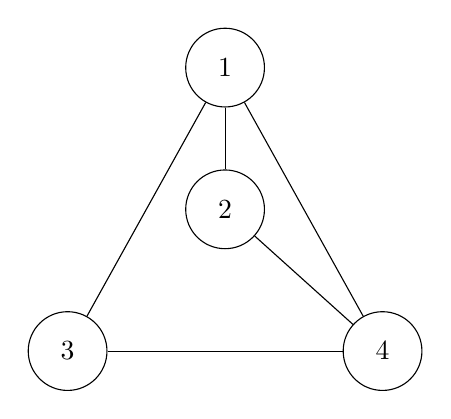
\begin{tikzpicture}[node distance = 1.8cm]
                        \node (1) [branchnode] {1};
                        \node (2) [branchnode, below of=1] {2};
                        \node (3) [branchnode, below of=2, xshift=-2cm] {3};
                        \node (4) [branchnode, below of=2, xshift=2cm] {4};
                        \draw (1) -- (2);
                        \draw (1) -- (3);
                        \draw (1) -- (4);
                        \draw (2) -- (4);
                        \draw (3) -- (4);
                    \end{tikzpicture}
                    \caption{Example of vertices packing problem}
                \end{figure}

                The PACK of this graph is

                \begin{equation*}
                    PACK = conv\left(
                        \left(\begin{matrix}0 \\ 0 \\ 0 \\ 0\end{matrix}\right),
                        \left(\begin{matrix}1 \\ 0 \\ 0 \\ 0\end{matrix}\right),
                        \left(\begin{matrix}0 \\ 1 \\ 0 \\ 0\end{matrix}\right),
                        \left(\begin{matrix}0 \\ 0 \\ 1 \\ 0\end{matrix}\right),
                        \left(\begin{matrix}0 \\ 0 \\ 0 \\ 1\end{matrix}\right),
                        \left(\begin{matrix}0 \\ 1 \\ 1 \\ 0\end{matrix}\right)
                        \right)\nonumber
                \end{equation*}

                The dimension of PACK, i.e. $dim(PACK(G))$ is (full-dimensional)
                \begin{equation*}
                    dim(PACK(G)) = |V| \nonumber
                \end{equation*}
                To prove that $dim(PACK(G)) = |V|$, we need to find $|V| + 1$ affinely independent vectors.\\
                \begin{proof}
                    \begin{equation*}
                        rank\left(\left[\begin{matrix}0 & I_{|V|} \\ 1 & 1\end{matrix}\right]\right) = |V| + 1 \nonumber
                    \end{equation*}
                \end{proof}                    
                Therefore, in PACK, $rank(A^=,b^=)=0$ 

            \paragraph{Inequalities and Facets of conv(VP) - Nonnegative Constraints}
                $x_i \ge 0$ induce facets.\\
                \begin{proof}
                    \begin{equation*}
                        rank\left(\left[\begin{matrix}0 & 0 \\ 0 & I_{|V|}\end{matrix}\right]\right) = |V| + 1 \nonumber
                    \end{equation*}    
                \end{proof}               

            \paragraph{Inequalities and Facets of conv(VP) - Neighborhood Constraints}
                $x_i + x_j \le 1$ is a valid constraint, but it \textbf{DOES NOT} always induce facet.

            \paragraph{Inequalities and Facets of conv(VP) - Odd Hole}
                Consider a graph $G=(V, E)$, the covering problem is
                \begin{equation*}
                    \sum_{e\in \delta(i)}x_e \le 1, i\in V, x_e\in \{0, 1\}, e\in E\nonumber
                \end{equation*}
                For $T\subset V$, denote $\delta(i)$ as all edges induce to $i\in V$, denote $E(T) \subset E$ as all the edges linked between $(i, j), i\in T, j\in T$, therefore we have
                \begin{equation*}
                    \sum_{i\in T}\sum_{e\in \delta(i)}x_e \le |T| \nonumber
                \end{equation*}
                For edges linking $i \in T, j \in T$, count them twice, for edges linking $i\in T, j\notin T$, count them once.We can have a new constraint
                \begin{equation*}
                    2\sum_{e\in E(T)}x_e + \sum_{e\in \delta(V\setminus T, T)}x_e \le |T| \nonumber
                \end{equation*}
                Perform the Gomory Cut, the following constraint is a valid:
                \begin{equation*}
                    \sum_{e\in E(T)}x_e \le \lfloor \frac{|T|}2 \rfloor \nonumber
                \end{equation*}

                $H$ is an odd hole if it contains circle of $k$ nodes, such that $k$ is odd and there is no cords. e.g. \{1, 2, 5, 6, 3\}. Then, the following inequality is valid,
                \begin{equation*}
                    \sum_{i\in H}x_i\le \frac{|H|-1}2 \nonumber
                \end{equation*}
                Odd Hole inequality \textbf{DOES NOT} always induce facets.

            \paragraph{Inequalities and Facets of conv(VP) - Maximum Clique}
                A \textbf{clique} is a subset of a graph that in the clique every two vertices linked with each other (complete sub-graph). A \textbf{maximum clique} is a clique that any other vertice can not form a clique with all the points in this clique.

                $C$ is a maximum clique, then the following inequality is valid and induce a facet,
                \begin{equation*}
                    \sum_{i\in C} x_i \le 1 \nonumber
                \end{equation*}
                
                \begin{proof}
                    First, if $C=V$
                    \begin{equation*}
                        rank\left(\left[I\right]\right) = |C| = |V| \nonumber           
                    \end{equation*}
                    Second, if $C$ is a subset of $V$, for each vertice in $V \setminus C$, there should be at least one vertice in $C$ that is not linked with it. Therefore for each vertice in $C$ we can find a packing.
                \end{proof}                    

        \subsection{Knapsack Problem}
            \paragraph{Knapsack Problem Formulation}
                Consider the knapsack set KNAP
                \begin{equation*}conv(KNAP)= conv(\{x\in \mathbb{B}^n|\sum_{j\in N}a_jx_j\le b\})\end{equation*}
                in where
                \begin{itemize}
                    \item $N = \{1, 2, ..., n\}$
                    \item With out lost of generality, assume that $a_j > 0, \forall j \in N$ and $a_j < b, \forall j \in N$
                \end{itemize}

            \paragraph{Valid Inequalities for a Relaxation}
                For $P=\{x\in \mathbb{B}^n | Ax\le b\}$, each row can be regard as a Knapsack problem, i.e. for row $i$
                \begin{equation*}
                    P_i = \{x\in \mathbb{B}^n | a_i^T x \le b_i\} 
                \end{equation*}
                is a relaxation of $P$, therefore,
                \begin{equation*}
                    P\subseteq P_i, \forall i=1,2,...,m 
                \end{equation*}
                \begin{equation*}
                    P\subseteq \cap_{i=1}^m P_i 
                \end{equation*}
                So any inequality valid for a relaxation of an IP is also valid for IP itself.
                
            \paragraph{Cover and Extended Cover}
                A set $C\subseteq N$ is a cover if $\sum_{j\in C} a_j > b$, a cover $C$ is minimal cover if
                \begin{equation*}
                    C\subseteq N | \sum_{j\in C}a_j>b, \sum_{j\in C\setminus k} a_j < b, \forall k \in C 
                \end{equation*}
                For a cover $C$, we can have the cover inequality
                \begin{equation*}
                    \sum_{j\in C}x_j \le |C|-1
                \end{equation*}
                The inequality is trivial considering the pigeonhole principle.\\
                $C\subseteq N$ is a minimal cover, then $E(C)$ is defined as following:
                \begin{equation*}
                    E(C) = C\cup \{j \in N | a_j \ge a_i, \forall i \in C\}
                \end{equation*}
                is called an extended cover. Then we have,
                \begin{equation*}
                    \sum_{i\in E(C)} x_i \le |C| - 1 \text{ dominates } \sum_{i\in C} x_i \le |C| - 1
                \end{equation*}
                and
                \begin{equation*}
                    \sum_{i\in E(C)} x_i \le |C| - 1 \text{ dominates } \sum_{i\in E(C)} x_i \le |E(C)| - 1
                \end{equation*}
                Hereby we need to prove that $\sum_{i\in E(C)} x_i \le |C| - 1$ is valid, by contradiction.\\
                \begin{proof}
                    Suppose $x^R \in KNAP$, $R$ is a feasible solution, Where
                    \begin{equation*}
                        x^R_j = \begin{cases}1, \quad \text{if $j\in R$} \\ 0, \quad \text{otherwise}\end{cases} 
                    \end{equation*}
                    Then
                    \begin{equation*}
                        \sum_{j\in E(C)}x^R_j \ge |C| \Rightarrow |R \cap E(C)| \ge |C|  
                    \end{equation*}
                    therefore
                    \begin{equation*}
                        \sum_{j\in R}a_j \ge \sum_{j\in R \cap E(C)} a_j \ge \sum_{j\in C} a_j > b 
                    \end{equation*}
                    which means $R$ is a cover, it is contradict to $\sum_{j\in E(C)}x^R_j \ge |C|$ so $x^R \notin KNAP$
                \end{proof}

            \paragraph{Dimension of KNAP}
                $conv(KNAP)$ is full dimension, i.e. $dim(conv(KNAP))=n$.\\
                \begin{proof}
                    $0, e_j, \forall j\in N$ are $n + 1$ affinely independent points in $conv(KNAP)$
                \end{proof}

            \paragraph{Inequalities and Facets of conv(KNAP) - Lower Bound and Upper Bound Constraints}
                \begin{itemize}
                    \item $x_k\ge 0$ is a facet of $conv(KNAP)$
                    \begin{proof}
                        $0, e_j, \forall j\in N\setminus k$ are $n$ affinely independent points that satisfied $x_k=0$
                    \end{proof}
                    \item $x_k\le 1$ is a facet iff $a_j + a_k \le b, \forall j\in N \setminus k$
                    \begin{proof}
                        $e_k, e_j+e_k, \forall j \in N\setminus k$ are $n$ affinely independent points that satisfied $x_k = 1$
                    \end{proof}
                \end{itemize}                

            \paragraph{Inequalities and Facets of conv(KNAP) - Extended Cover}
                Order the variables so that $a_1 \ge a_2 \ge \dots \ge a_n$, therefore $a_1 = a_{max}$\\
                Let $C$ be a cover with $\{j_1, j_2, \dots, j_r\}$ where $j_1 < j_2 < \dots < j_r$ so that $a_{j_1} \ge a_{j_2} \ge \dots \ge a_{j_r}$\\
                Let $p = \min\{j | j\in N \setminus E(C)\}$\\
                Then
                \begin{equation*}
                    \sum_{j\in E(C)} x_j \le |C| - 1 
                \end{equation*}
                is a facet of $conv(KNAP)$ if
                \begin{itemize}               
                    \item$C = N$\\
                    \begin{proof}
                        \begin{equation*}
                        R_k = C\setminus k, \forall k \in C = N \setminus k, \forall k \in N 
                    \end{equation*}
                    have $|N|$ affinely independent vectors
                    \end{proof}                
                    \item$E(C) = N$ and $\sum_{j\in C \setminus \{j_1, j_2\}} a_j + a_{max} \le b$\\
                    \begin{proof}
                         ($j_1, j_2$ are two heaviest elements in $C$)
                        \begin{equation*}
                            S_k = C\setminus \{j_1, j_2\}\cup \{k\}, \forall k\in E(C)\setminus C 
                        \end{equation*}
                        $R_k\cup S_k$ have $|C|+|E(C) \setminus C| = |E(C)| = |N|$ affinely independent vectors
                    \end{proof} 
                    \item$C = E(C)$ and $\sum_{j\in C \setminus j_1} a_j + a_p \le b$)\\
                    \begin{proof}
                        ($j_1$ is the heaviest element in $C$, $k$ is the lightest element outside extended cover)
                        \begin{equation*}
                            T_k = C \setminus j_i \cup \{k\}, \forall k\in N\setminus E(C) 
                        \end{equation*}
                        $R_k \cup T_k$ have $|N \setminus E(C)| + |E(C)| = |N\setminus C| + |C| = |N|$  affinely independent vectors
                    \end{proof}
                    \item$C \subset E(C) \subset N$ and $\sum_{j\in C \setminus \{j_1, j_2\}} a_j + a_{max} \le b$ and $\sum_{j\in C \setminus j_1} a_j + a_p \le b$\\
                    \begin{proof}
                        $S_k \cup T_k$ have $|E(C) \setminus C| + |N \setminus E(C)| = |N|$ affinely independent vectors
                    \end{proof}
                \end{itemize}

    \section{Generic Cutting Planes}
        \subsection{General Approach}
            \paragraph{Cutting Planes}
            \begin{itemize}
                \item Cutting planes are referred to inequalities valid for $conv(S)$, but which is violated by the solution obtained by solving the current LP relaxation.
                \item Cutting plane methods attempt to improve the bound produced by the LP relaxation by iteratively adding cutting planes to the initial LP relaxation.
                \item Adding such inequalities to the LP relaxation may improve the bound (this is not a guarantee).
            \end{itemize}

            \paragraph{Separation Problem} Given a polygon $P \in \mathbb{R}^n$ and $\mathbf{x}^* \in \mathbb{R}^n$, determine whether $\mathbf{x}^* \in P$, and if not, determine $(\mathbf{\pi}, \pi_0)$, a valid inequality for $P$ such that $\mathbf{\pi} \mathbf{x}^* \ge \pi_0$

        \subsection{Generic Cutting Planes}
            \paragraph{Observation}
                For integer program over a set of variables $x_1, x_2, \cdots, x_n \in \mathbb{Z}_+$
                \begin{itemize}
                    \item If $\mathbf{ax} = \mathbf{b}$ is a constraint of $P$, then $\mathbf{ax \le b}$ is a valid constraint of $P$
                    \item Suppose there are two valid constraints
                        \begin{align*}
                            a_{11} x_1 + a_{12} x_2 + \cdots + a_{1n} x_n \le b_1
                        \end{align*}
                        and
                        \begin{align*}
                            a_{21} x_2 + a_{22} x_2 + \cdots + a_{2n} x_n \le b_2
                        \end{align*}
                        then
                        \begin{align*}
                            & u_1 (a_{11} x_1 + a_{12} x_2 + \cdots + a_{1n} x_n)\\
                          + & u_2 (a_{21} x_2 + a_{22} x_2 + \cdots + a_{2n} x_n) \\
                            & \qquad \qquad \qquad \qquad \qquad \le u_1 b_1 + u_2 b_2
                        \end{align*}
                        is a valid inequality for $P$
                    \item If $a \le b$ and $a$ is an integer number, then $a \le \floor{b}$
                    \item $x_i \in \mathbb{Z}_+ \Rightarrow -x_i \le 0$
                    \item WLOG, assume $\forall a_i$ in constraint $\sum_{i=1}^n a_i x_i \le b$, $a_i$ is a fractional number. Let $f_i = a_i - \floor{a_i}$ be the fractional part, and $f_i \ge 0$. Then,
                    \begin{equation*}
                        \sum_{i=1}^n a_i x_i - \sum_{i=1}^n f_i x_i \le b - 0
                    \end{equation*}
                    $\Rightarrow$
                    \begin{equation*}
                        \sum_{i=1}^n \floor{a_i} x_i \le \floor{b}
                    \end{equation*} is a valid inequality for $P$.
                \end{itemize}
                
            \paragraph{Chv\'atal-Gomory Rounding Method}
                Let $X = P \cap \mathbb{Z}^n$ be the feasible set of an integer program, where
                \begin{equation*}
                    P = \{\mathbf{x} \in \mathbb{R}^n | \mathbf{Ax}\le \mathbf{b}, \mathbf{x} \ge 0\}
                \end{equation*}
                Also let $\mathbf{a}_i$ be the $i$th column of $\mathbf{A}$, then
                \begin{equation*}
                    \sum_{i = 1}^n \mathbf{u} \mathbf{a}_i x_i \le \mathbf{ub}
                \end{equation*}
                is a valid inequality for $P$ for $u \ge 0$, then
                \begin{equation*}
                    \sum_{i = 1}^n \floor{\mathbf{u} \mathbf{a}_i} x_i \le \mathbf{ub}
                \end{equation*}
                is a valid inequality for $P$, then
                \begin{equation*}
                    \sum_{i = 1}^n \floor{\mathbf{u} \mathbf{a}_i} x_i \le \floor{\mathbf{ub}}
                \end{equation*}
                is a valid inequality for $P$, since $x_i$ is an integer. Such procedures are called Chv\'atal-Gomory rounding procedure, and such cuts are called Chv\'atal-Gomory Cuts.

            \paragraph{Example 1}
                Let $P$ be
                \begin{align*}
                    2 x_1 + 3 x_2 &\le 5\\
                    -x_1 + x_2 &\le 2\\
                    x_1, x_2 &\ge 0
                \end{align*}
                Then
                \begin{equation*}
                    \mathbf{A} = \begin{bmatrix}2 & 3 \\ -1 & 1\end{bmatrix} \Rightarrow \mathbf{a}_1 = \begin{bmatrix}2 \\ -1\end{bmatrix}, \mathbf{a}_2 = \begin{bmatrix}3 \\ 1\end{bmatrix}
                \end{equation*}
                Let
                \begin{equation*}
                    \mathbf{u} = \begin{bmatrix}1/2 & 1/3\end{bmatrix}
                \end{equation*},
                then
                \begin{equation*}
                    \begin{bmatrix}1/2 & 1/3\end{bmatrix} \begin{bmatrix}2 \\ -1\end{bmatrix} x_1 + \begin{bmatrix}1/2 & 1/3\end{bmatrix} \begin{bmatrix}3 \\ 1\end{bmatrix} x_2 \le \begin{bmatrix}1/2 & 1/3\end{bmatrix} \begin{bmatrix}5 \\ 2\end{bmatrix}
                \end{equation*}
                which is
                \begin{equation*}
                    \frac{2}{3} x_1 + \frac{11}{6} x_2 \le \frac{19}{6}
                \end{equation*}
                then, 
                \begin{equation*}
                    \floor{\frac{2}{3}} x_1 + \floor{\frac{11}{6}} x_2 \le \floor{\frac{19}{6}} \Rightarrow x_2 \le 3
                \end{equation*}

            \paragraph{Example 2}
                Let $P$ be
                \begin{align*}
                    7 x_1 - 2x_2 &\le 14\\
                    x_2 &\le 3\\
                    2 x_1 - 2x_2 &\le 3\\
                    x_1, x_2 &\ge 0
                \end{align*}

                Let $u = \begin{bmatrix}\frac{2}{7} & \frac{37}{63} & 0\end{bmatrix}$

                Then $2 x_1 + \frac{1}{63} x_2 \le \frac{185}{21} \Rightarrow x_1 \le 4$

            \paragraph{Observation}
                \begin{itemize}
                    \item It is possible to generate $conv(X)$ using C-G procedures
                    \item The crux lies on the choice of $\mathbf{u}$
                    \item The number of iterations can be huge
                    \item Nevertheless, the procedure has been proven to work well in practice in recent years to generate good inequalities
                    \item One can try generating random multipliers and test the method
                \end{itemize}

        \subsection{Gomory Cuts}
            Gomory cutting planes can also be derived directly from the tableau while solving an LP relaxation. Consider the set
            \begin{equation*}
                P = \{(\mathbf{x, s}) \in \mathbb{Z}_+^{n + m}| \mathbf{Ax + Is = b}\}
            \end{equation*}
            in which the LP relaxation of an ILP is put in standard form. Assume for $A$, all the coefficients are integers, so that the slack variables are integers. Clearly,
            \begin{equation*}
                \mathbf{B^{-1}Ax + B^{-1}Is = B^{-1}b}
            \end{equation*}
            Let $\mathbf{\lambda} = \mathbf{B^{-1}}_j$, then we obtain
            \begin{equation*}
                \sum_{j = 1}^n \mathbf{\lambda A_j} x_j + \sum_{i = 1}^m \mathbf{\lambda}_i s_i = \mathbf{\lambda b}
            \end{equation*}
            where $\mathbf{A}_j$ is the $j$th column of $\mathbf{A}$ and $\mathbf{\lambda}$ is a row if $\mathbf{B}^{-1}$. Then, the Gomory cut is define by
            \begin{equation*}
                \sum_{j = 1}^n (\mathbf{\lambda A}_j - \floor{\mathbf{\lambda A}_j}) x_j + \sum_{i = 1}^m (\mathbf{\lambda}_i - \floor{\mathbf{\lambda}_i}) s_i \ge \mathbf{\lambda b} - \floor{\mathbf{\lambda b}}
            \end{equation*}
            Gomory cut is a Chv\'atal-Gomory cut with weights $\mathbf{u}_i = \mathbf{\lambda}_i - \floor{\mathbf{\lambda}_i}$.

            \paragraph{Example}
                For the following IP
                \begin{align*}
                    \max \quad & 2 x_1 + 5 x_2\\
                    \text{s.t.} \quad & 4 x_1 + x_2 \le 28\\
                    & x_1 + 4 x_2 \le 27\\
                    & x_1 - x_2 \le 1\\
                    & x_1, x_2 \in \mathbb{Z}_+
                \end{align*}

                The optimal tableau of the LP relaxation is as follows

                \begin{table}[H]
                    \centering
                    \begin{tabular}{c|ccccc|c}
                        & $x_1$ & $x_2$ & $s_1$ & $s_2$ & $s_3$ & RHS\\
                        \hline
                        $x_2$ & 0 & 1 & -2/30 & 8/30 & 0 & 16/3\\
                        $s_3$ & 0 & 0 & -1/3 & 1/3 & 1 & 2/3\\
                        $x_1$ & 1 & 0 & 8/30 & -2/30 & 0 & 17/3
                    \end{tabular}
                \end{table}

                For the first row, the Gomory cut is
                \begin{equation*}
                    \frac{28}{30} s_1 + \frac{8}{30} s_2 \ge \frac{1}{3}
                \end{equation*}
                Replace the slack variables, we have
                \begin{equation*}
                    4 x_1 + 2 x_2 \le 33
                \end{equation*}

                For the second row, the Gomory cut is
                \begin{equation*}
                    \frac{2}{3} s_1 + \frac{1}{3} s_2 \le \frac{2}{3}
                \end{equation*}

                Replace the slack variables, we have
                \begin{equation*}
                    3 x_1 + 2 x_2 \le 27
                \end{equation*}

                For the third row, the Gomory cut is
                \begin{equation*}
                    \frac{8}{30}s_1 + \frac{28}{30}s_2 \ge \frac{2}{3}
                \end{equation*}

                Replace the slack variables, we have
                \begin{equation*}
                    x_1 + 2 x_2 \le 16
                \end{equation*}

                This picture shows the effect of adding all Gomory cuts in the first round
                \begin{figure}[!h]
                    \centering
                    \includegraphics[width=0.6\textwidth]{../../image/CG.png}
                \end{figure}

    \section{Branch and Cut}
        \paragraph{Two types of valid inequalities}
            The structural constraints are 
            \begin{itemize}
                \item while this is not a standard term used in mathematical programming, we will use it in reference to the constraints that define a formulation
                \item these are constraints needs to define the problem. If removed, some infeasible integer solutions may become part of the solution space
            \end{itemize}

            The cutting planes are
            \begin{itemize}
                \item these are valid constraints that are not needed to define the problem but can be added to tighten the LP relaxation of a formulation
                \item in other words, they are used for trying to obtain a better LP bound
            \end{itemize}

        \paragraph{User cuts}


            \begin{figure}[H]
                \centering
                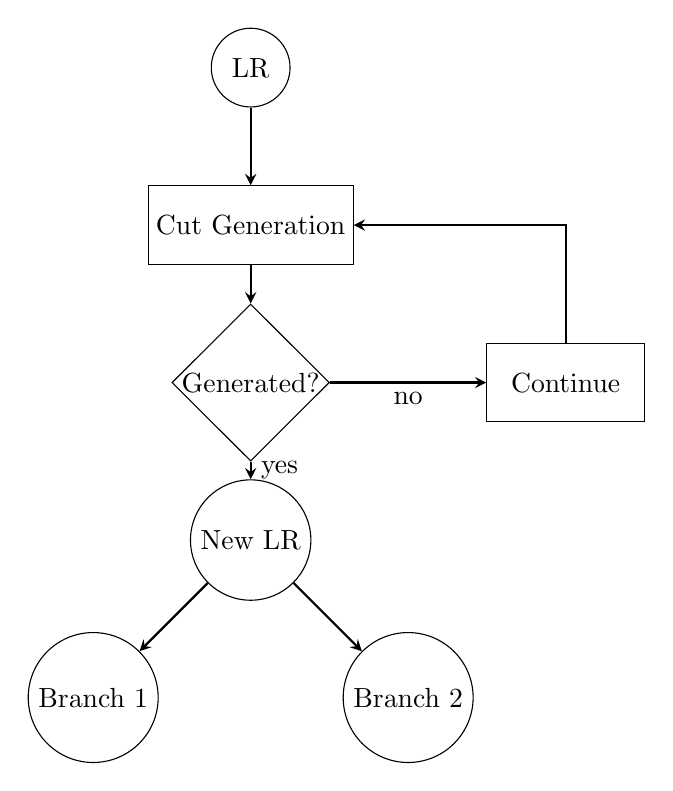
\begin{tikzpicture}[node distance = 2cm]
                    \node (LR) [branchnode] {LR};
                    \node (CG) [process, below of=LR] {Cut Generation};
                    \node (CLimit) [decision, below of=CG] {Generated?};
                    \node (Cont) [process, below of=CG, xshift=4cm] {Continue};
                    \node (NLR) [branchnode, below of=CLimit] {New LR};
                    \node (LNLR) [branchnode, below of=NLR, xshift=-2cm] {Branch 1};
                    \node (RNLR) [branchnode, below of=NLR, xshift=2cm] {Branch 2};
                    \draw [arrow] (LR) -- (CG);
                    \draw [arrow] (CG) -- (CLimit);
                    \draw [arrow] (CLimit) -- node [right] {yes} (NLR);
                    \draw [arrow] (CLimit) -- node [below] {no} (Cont);
                    \draw [arrow] (Cont) |- (CG);
                    \draw [arrow] (NLR) -- (LNLR);
                    \draw [arrow] (NLR) -- (RNLR);
                \end{tikzpicture}
                \caption {Branch and Cut for Optional Inequality}\label{OptInq}
            \end{figure}

            Consider the vertice packing problem, we have mentioned that the maximum cliques can be used for adding valid inequalities, this is how it works

            \begin{itemize}
                \item Given a fractional solution $\hat{x}$, we can find a clique for which $\sum_{i \in C} x_i \le 1, C \in Clique(G)$ is violated
                \item Solve the following separation problem
                \begin{align*}
                    \max \quad & \gamma = \sum_{i \in V} \hat{x}_i z_i\\
                    \text{s.t.} \quad & z_i + z_j \le 1, \{i, j\} \notin E\\
                    &z_i \in \{0, 1\}, i \in V
                \end{align*}
                \item if $\gamma > 1$ add the clique cut associate with $C$.
            \end{itemize}

        \paragraph{Lazy cuts}
            A typical example for lazy cuts is the DFJ sub-tour elimination for TSP. We will discuss later in this semester.

            \begin{figure}[H]
                \centering
                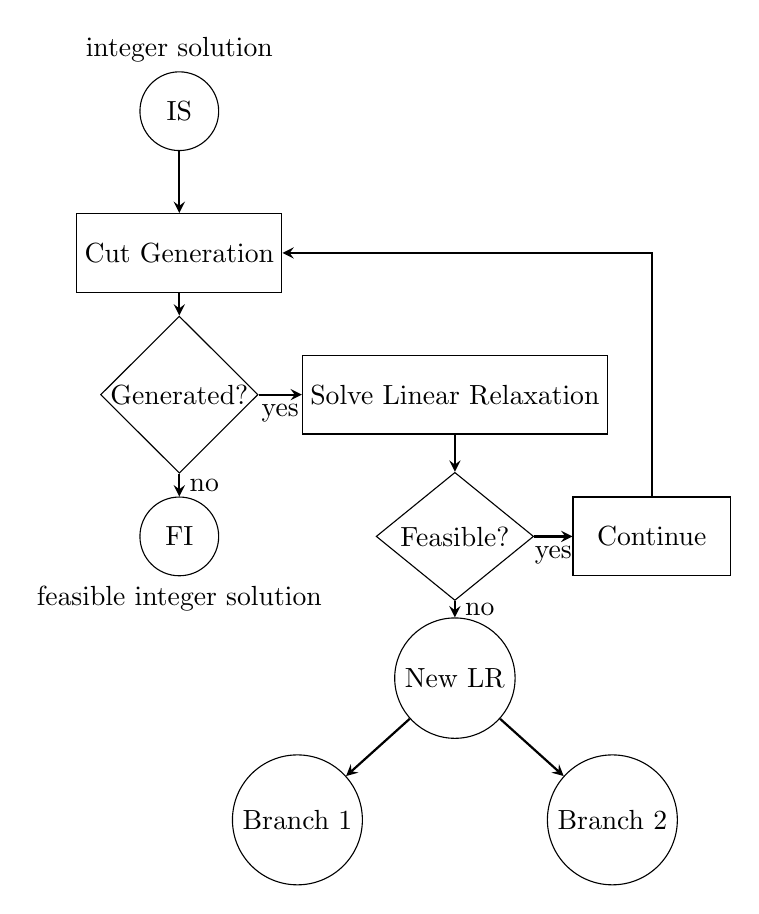
\begin{tikzpicture}[node distance = 1.8cm]
                    \node (IS) [branchnode, label = above:integer solution] {IS};
                    \node (CG) [process, below of=IS] {Cut Generation};
                    \node (CLimit) [decision, below of=CG] {Generated?};
                    \node (FI) [branchnode, below of=CLimit, label = below:feasible integer solution] {FI};
                    \node (LP) [process, below of=CG, xshift = 3.5cm] {Solve Linear Relaxation};
                    \node (LPF) [decision, below of=LP] {Feasible?};
                    \node (NLR) [branchnode, below of=LPF] {New LR};
                    \node (LNLR) [branchnode, below of=NLR, xshift=-2cm] {Branch 1};
                    \node (RNLR) [branchnode, below of=NLR, xshift=2cm] {Branch 2};
                    \node (Cont) [process, below of=LP, xshift=2.5cm] {Continue};
                    \draw [arrow] (IS) -- (CG);
                    \draw [arrow] (CG) -- (CLimit);
                    \draw [arrow] (CLimit) -- node [right] {no} (FI);
                    \draw [arrow] (CLimit) -- node [below] {yes} (LP);
                    \draw [arrow] (LP) -- (LPF);
                    \draw [arrow] (LPF) -- node [right] {no} (NLR);
                    \draw [arrow] (LPF) -- node [below] {yes} (Cont);
                    \draw [arrow] (NLR) -- (LNLR);
                    \draw [arrow] (NLR) -- (RNLR);
                    \draw [arrow] (Cont) |- (CG);
                \end{tikzpicture}
                \caption {Branch and Cut for Essential Inequality}\label{EssInq}
            \end{figure}

\end{document}